%%%%%%%%%%%%%%%%%%%%%%%%%%%%%%%%%%%%%%%%%%%%%%%%%%%%%%%%%%%%%%%%%%%%%%%%%%%%%%%%%%%%%%%%
\chapter{Kitaev Honeycomb Model}
\label{chapter:KitaevHoneycombModel}
%%%%%%%%%%%%%%%%%%%%%%%%%%%%%%%%%%%%%%%%%%%%%%%%%%%%%%%%%%%%%%%%%%%%%%%%%%%%%%%%%%%%%%%%
%
%
This chapter discusses in greater detail the Kitaev honeycomb model which was introduced in Chapter~\ref{chapter:Introduction}.
Kitaev published his now famous quantum spin-1/2 model in 2006~\cite{KitaevAoP2006}.
There was no clear solid state realization of the model in mind at the time, however, it regardless proved to be a very useful case study of fractionalization and quantum spin liquids as it was a rare example of an exactly solvable model of frustrated, interacting quantum spins.
As will be discussed in Chapter~\ref{chapter:TransitionMetalOxides}, the model was eventually shown to be relevant in the description of certain spin-orbit entangled $J_{\rm eff} = 1/2$ Mott insulators~\cite{JackeliPRL2009}, breathing new life into the field driven by the search for such materials.

The model, defined in Eq.~\eqref{eq:chapter02_KitaevHamiltonian} in the next section, describes quantum spin-1/2 degrees of freedom located at the sites of a honeycomb lattice which interact via Ising-like exchange, the quantization axis of which depends on the direction of the bond connecting the two spins.
The competition of incompatible local Ising constraints results in a strong exchange frustration.
Rather surprisingly, the model may be solved exactly by a mapping of spins to Majorana fermions, resulting in a theory of Majorana fermions coupled to a static \ZZ~gauge field.

Depending on the choice of exchange couplings, the ground state of the model is either a gapped or gapless quantum spin liquid with extremely short-ranged spin-spin correlations.
The gapped spin liquid phase has been shown to be equivalent to the toric code model (also introduced by Kitaev) which hosts gapped, Abelian anyon excitations~\cite{KitaevAoP2003,KitaevAoP2006}.
With the exception of Appendix~\ref{appendix:LoopModels}, this thesis does not treat the gapped portion of the ground state phase diagram in any great detail.
Instead, the focus here is on the \textit{gapless} spin liquid phase which is found when all exchange couplings are of roughly equal strength.
In this phase, in addition to gapped \ZZ~flux excitations one finds gapless Dirac fermion quasiparticles.
Under application of a magnetic field, the fermions are also gapped out, resulting in a topological Chern insulator phase, the excitations of which are non-Abelian anyons.

The remainder of this chapter is structured as follows.
In Section~\ref{section:chapter02_Definition}, the model is defined and a macroscopic number of conserved quantities are identified.
Section~\ref{section:chapter02_Z2GaugeTheory} explains the details of mapping the original spin model to one of Majorana fermions coupled to a static \ZZ~gauge field.
Section~\ref{section:chapter02_GeneralAspects} shows how the exact solution of the model follows from the aforementioned mapping and in Section~\ref{section:chapter02_GroundstatePhaseDiagram} the model is explicitly solved throughout its ground state phase diagram.
In Section~\ref{section:chapter02_WeakMagneticField}, the effects of time-reversal symmetry breaking are discussed in the concrete context of an applied magnetic field.
Finally, Section~\ref{section:chapter02_Summary} provides a brief summary.


%
%
%%%%%%%%%%%%%%%%%%%%%%%%%%%%%%%%%%%%%%%%%%%%%%%%%%%%%%%%%%%%%%%%%%%%%%%%%%%%%%%%%%%%%%%%
\section{Definition of the model}
\label{section:chapter02_Definition}
%%%%%%%%%%%%%%%%%%%%%%%%%%%%%%%%%%%%%%%%%%%%%%%%%%%%%%%%%%%%%%%%%%%%%%%%%%%%%%%%%%%%%%%%
%
%
%
\begin{figure}[tb]
	\centering
	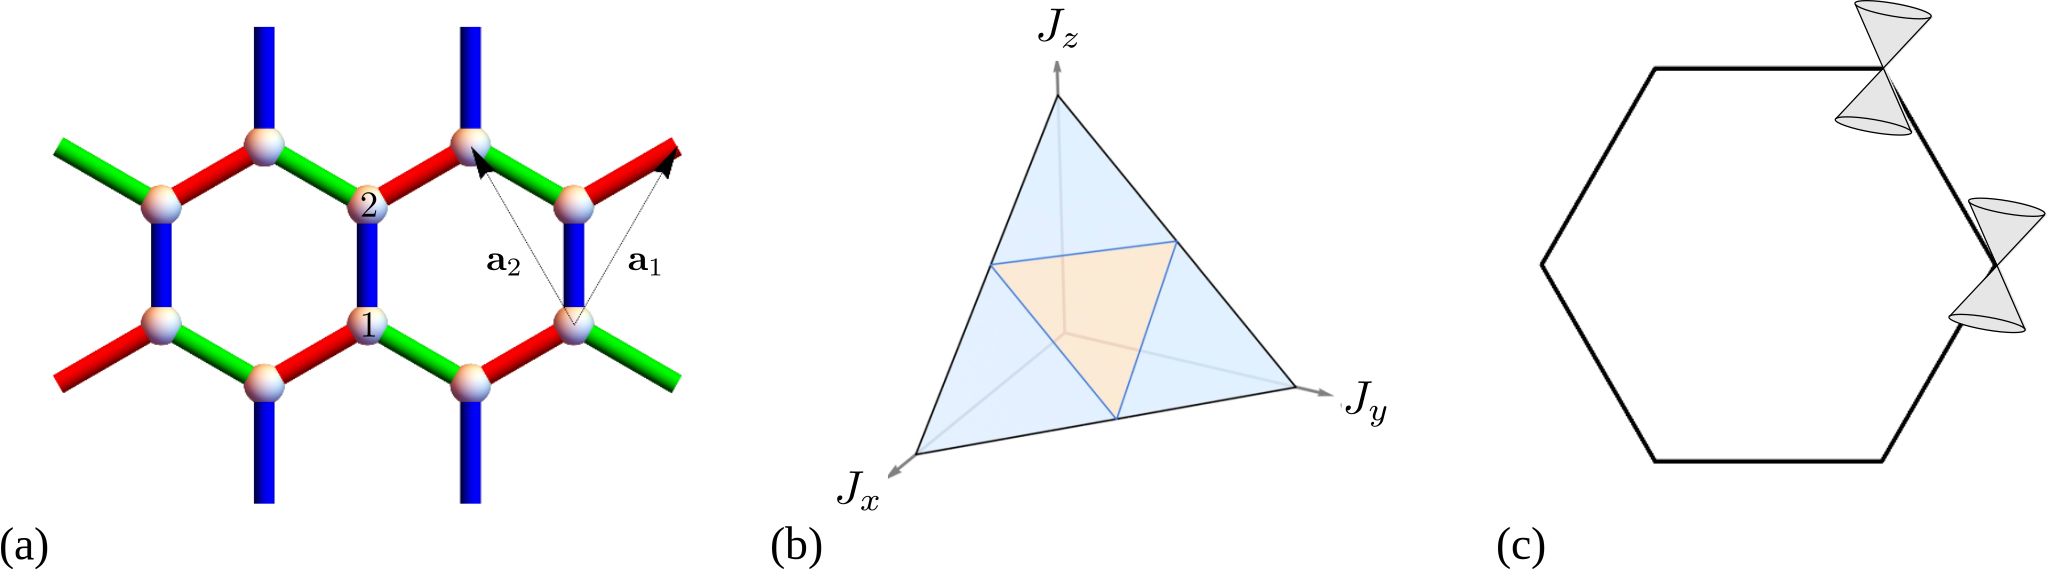
\includegraphics[width=\linewidth]{./chapter02/HoneycombPanel.pdf}
	\caption{
		(a) Unit cell and lattice vectors for the Kitaev model on the honeycomb lattice.
		Red, green and blue colored links correspond to $x$-, $y$- and $z$-type bonds, respectively.
		(b) Ground state phase diagram of the Kitaev model on the honeycomb lattice ($J_x + J_y + J_z = 1$).
		The blue regions correspond to gapped spin liquid phases, whereas the orange region corresponds to the gapless spin liquid phase.
		(c) Visualization of the Dirac cones for isotropic coupling.
	}
	\label{fig:chapter02_HoneycombPanel}
\end{figure}
%
The Kitaev model describes a system of interacting quantum spin-$1/2$ moments located at the vertices of a two-dimensional honeycomb lattice and is governed by the Hamiltonian
%
\begin{equation}
	\op{H}_{\rm Kitaev} = -J_x \sum_{x {\rm -links}} \sigma_j^x \sigma_k^x - J_y \sum_{y {\rm -links}} \sigma_j^y \sigma_k^y - J_z \sum_{z {\rm -links}} \sigma_j^z \sigma_k^z,
	\label{eq:chapter02_KitaevHamiltonian}
\end{equation}
%
where the summations are over nearest neighbor spins $\avg{j,k}$ with each link counted exactly once, the exchange couplings are chosen to be ferromagnetic, \ie, $J_{\gamma} \geq 0$, and each link connecting the spins is assigned to be of type $x$, $y$ or $z$.
The assignment of bond types is given in Figure~\ref{fig:chapter02_HoneycombPanel}~(a), where red, green and blue colored links correspond to $x$-, $y-$ and $z-$type bonds, respectively.
The Hamiltonian~\eqref{eq:chapter02_KitaevHamiltonian} may be written more compactly as
%
\begin{equation}
	\op{H}_{\rm Kitaev} = -\sum_{\gamma {\rm -links}} J_{\gamma}~\sigma_j^{\gamma} \sigma_k^{\gamma}.
	\label{eq:chapter02_KitaevHamiltonianCompact}
\end{equation}
%

The spins interact with their nearest neighbors via an Ising-like exchange, however, the component of the spin which is coupled depends on the type of bond connecting the neighboring spins.
This directional dependence of the exchange makes it impossible for a given spin to satisfy all of its neighbors simultaneously and results in a highly frustrated lattice of spins.
Despite describing a system of strongly interacting and highly frustrated quantum spins, the model is exactly solvable due to the combination of it possessing an extensive number of conserved quantities along with a clever representation of the Pauli matrices in terms of Majorana operators.

The first step to solving the model is the identification of conserved quantities.
For each hexagonal plaquette $p$ in the lattice, one may define a product of spins around the corresponding closed loop as
%
\begin{equation}
	\op{W}_p = -\prod_{\avg{j,k}\in p} \left(-i \sigma_j^{\gamma} \sigma_k^{\gamma}\right),
	\label{eq:chapter02_SpinLoopOperator}
\end{equation}
%
where the product is understood to occur in the counter-clockwise sense around the loop.
All such loop operators commute with each other as well as with the Hamiltonian~\eqref{eq:chapter02_KitaevHamiltonianCompact} and, thus, represent an extensive number of conserved quantities.
As such, they serve to partition the Hilbert space of the spins into sectors corresponding to the set of eigenvalues $\{w_p\}$.
The loop operators can be shown to be both Hermitian and unitary and, thus, have eigenvalues $w_p = \pm 1$.
These loop operators will later be seen to correspond to the fluxes of a \ZZ~gauge field and the eigenspaces $\{w_p\}$ will be referred to as "flux" sectors.

As the definition of the loop operator in Eq.~\eqref{eq:chapter02_SpinLoopOperator} differs from that usually encountered in the literature, note that it is chosen in order to maintain consistency when working with lattices other than the honeycomb.
The factors of $i$ act to ensure that the operator $\op{W}_p$ is Hermitian no matter the length of the plaquette, whereas the choice of minus signs will be seen in Section~\ref{section:chapter02_Z2GaugeTheory} to fix a consistent relationship with the fluxes of the aforementioned \ZZ~gauge theory.
Note that for a loop of even length, the loop operator is even under time-reversal, whereas for a loop of odd length, the loop operator is odd under time-reversal.
This implies that any fixed flux eigenstate of a Kitaev Hamiltonian defined on a \textit{non}-bipartite lattice spontaneously breaks time-reversal symmetry as it necessarily specifies the fluxes through plaquettes of odd length.

One can already identify some properties of the eigenstates of Hamiltonian~\eqref{eq:chapter02_KitaevHamiltonianCompact} from flux conservation.
Any spin component $\sigma_j^{\gamma}$ anti-commutes with exactly two loop operators.
This implies that the application of a spin operator mixes orthogonal flux sectors, resulting in a vanishing spin expectation value $\avg{\sigma_j^{\gamma}} = 0$ for all sites of the lattice.
This further implies that all two-spin correlation functions must vanish unless the application of the second spin removes (reintroduces) the fluxes introduced (removed) by the first~\cite{BaskaranPRL2007}.
This happens only for on-site correlation functions and for nearest neighbor correlation functions of the form $\avg{\sigma_j^{\gamma} \sigma_k^{\gamma}}$, where sites $j, k$ are connected by a link of type $\gamma$.
These relations hold for \textit{all} eigenstates of the Hamiltonian.
Thus, the ground state of the Kitaev Hamiltonian~\eqref{eq:chapter02_KitaevHamiltonianCompact} has vanishing magnetization and (extremely) short-ranged spin-spin correlations as a quantum spin liquid should.


%
%
%%%%%%%%%%%%%%%%%%%%%%%%%%%%%%%%%%%%%%%%%%%%%%%%%%%%%%%%%%%%%%%%%%%%%%%%%%%%%%%%%%%%%%%%
\section{\texorpdfstring{\ZZ}{Z2}~gauge theory description}
\label{section:chapter02_Z2GaugeTheory}
%%%%%%%%%%%%%%%%%%%%%%%%%%%%%%%%%%%%%%%%%%%%%%%%%%%%%%%%%%%%%%%%%%%%%%%%%%%%%%%%%%%%%%%%
%
%
While the identification of conserved fluxes is a step in the right direction, it does not provide a complete solution to the problem.
In order to solve the model, it will be necessary to introduce an alternate representation of the spin-$1/2$ operators.
In this presentation, the solution originally introduced by Kitaev \cite{KitaevAoP2006} will be used.
There do exist, however, several other representations which have been used to solve this problem including Jordan-Wigner transformation \cite{FengPRL2007}, $SU(2)$ slave fermion representation \cite{BurnellPRB2011} as well as \textit{other} Majorana representations \cite{Tsvelik2003,YouPRB2012,SeifertPRBFeb2018,SeifertPRBOct2018} (as will be discussed in Chapter~\ref{chapter:ProjectiveSymmetryGroup}), each of which has its own strengths and weaknesses depending upon the desired application.

The approach used here will be to introduce four Majorana operators $c^{\gamma}$ at each site of the lattice, where $\gamma = 0,x,y,z$ (the superscript for $c^0$ will be dropped for notational convenience and readability wherever it does not hinder clarity).
These Majorana operators satisfy the usual Clifford algebra relations
%
\begin{equation}
	\{c_j^{\mu}, c_k^{\nu}\} = 2\delta^{\mu\nu}\delta_{jk}.
\end{equation}
%
Note that the Hilbert space of the Majorana operators at a given site is twice as large as that of the corresponding spin-$1/2$ operator.
One may introduce operators that act on this extended space
%
\begin{equation}
	\til{\sigma}_j^\mu = i c_j^{\mu} c_j \qquad (\mu = x,y,z)
	\label{eq:chapter02_ExtendedSpinOperators}
\end{equation}
%
which satisfy the same algebraic relations as the Pauli matrices \textit{when acting on physical states}.
The definition of extended spin-$1/2$ operators in Eq.~\eqref{eq:chapter02_ExtendedSpinOperators} is seen to possess a local \ZZ~gauge redundancy $c_j^\gamma \mapsto -c_j^\gamma$.
The physical Hilbert space is defined by those states satisfying $\op{D}_j = 1$ for all sites $j$, where the operator $\op{D}_j = c_j^x c_j^y c_j^z c_j$ represents the \ZZ~gauge transformation at site $j$, \ie,
%
\begin{equation}
	\{\op{D}_j, c_j^{\gamma}\} = 0.
\end{equation}
%

Replacing the spin operators of the original Hamiltonian~\eqref{eq:chapter02_KitaevHamiltonianCompact} with those in the extended space, one obtains a Hamiltonian of interacting Majorana fermions
%
\begin{equation}
	\op{H} = -\sum_{\avg{j,k}_{\gamma}} J_{\gamma}~(i c_j^{\gamma} c_j) (i c_k^{\gamma} c_k).
	\label{eq:chapter02_InteractingFermionHamiltonian}
\end{equation}
%
Defining link operators $\op{u}_{jk} = -\op{u}_{kj} = i c_j^{\gamma} c_k^{\gamma}$ on every link $\avg{j,k}_{\gamma}$, the Hamiltonian may be written\footnote{The $\dag$ has been included in the Hamiltonian in order to make the definition of the gauge transformations consistent.}
%
\begin{equation}
	\op{H} = i \sum_{\avg{j,k}_{\gamma}} J_{\gamma}~c\dag_j~\op{u}_{jk}~c_k
	\label{eq:chapter02_KitaevHamiltonianZ2}
\end{equation}
%
where it is easily seen to be invariant under local \ZZ~gauge transformations\linebreak $\op{G}_j \in \{\id_j,\op{D}_j\}$:
%
\begin{align}
	c_j &\rightarrow \op{G}_j c_j \nonumber\\
	\op{u}_{jk} &\rightarrow \op{G}_j \op{u}_{jk} \op{G}_k.
\end{align}
%
Of note is that the link operators commute with each other as well as with the Hamiltonian~\eqref{eq:chapter02_InteractingFermionHamiltonian} and represent conserved quantities.
Thus, they may serve to partition the extended Hilbert space into sectors corresponding to their eigenvalues $u_{jk}$.
As these operators are Hermitian and unitary, their eigenvalues $u_{jk} = \pm 1$.
Furthermore, replacing the spins in the definition of the loop operators $\op{W}_p$ to act in the extended space, one finds
%
\begin{align}
	\op{\til{W}}_p	&= -i^{|p|}\prod_{\avg{j,k}\in p} i \op{u}_{jk} \nonumber\\
				&= -i^{|p|} e^{i \op{\Phi}_p},
\end{align}
%
where $|p|$ denotes the length of the loop (for the honeycomb lattice considered here, $|p| = 6$) and $\op{\Phi}_p$ is the \ZZ-flux through the plaquette, establishing $\op{u}_{jk}$ as elements of a static \ZZ~gauge field where the loop operators $\op{W}_p$ correspond to the gauge-invariant fluxes of the gauge field.

In light of this interpretation, Hamiltonian~\eqref{eq:chapter02_KitaevHamiltonianZ2} may now be viewed as describing Majorana fermions hopping in the background of a static \ZZ~gauge field.
In principle, the \ZZ~gauge variables may be replaced by a static configuration and the resulting quadratic Hamiltonian diagonalized.
However, if one wishes to solve for the ground state, then the flux configuration of the ground state must first be determined.
Only then may a compatible gauge configuration be fixed and the Hamiltonian solved.


%
%
%%%%%%%%%%%%%%%%%%%%%%%%%%%%%%%%%%%%%%%%%%%%%%%%%%%%%%%%%%%%%%%%%%%%%%%%%%%%%%%%%%%%%%%%
\section{General aspects of the solution}
\label{section:chapter02_GeneralAspects}
%%%%%%%%%%%%%%%%%%%%%%%%%%%%%%%%%%%%%%%%%%%%%%%%%%%%%%%%%%%%%%%%%%%%%%%%%%%%%%%%%%%%%%%%
%
%
In order to solve for the ground state of Hamiltonian~\eqref{eq:chapter02_KitaevHamiltonianZ2}, one wishes to fix a gauge configuration and diagonalize the resulting quadratic Hamiltonian.
This gauge configuration must be constrained to yield the flux configuration of the ground state, making it necessary to first determine this ground state \textit{flux} configuration.
The most obvious way forward is a brute force numerical evaluation of possible flux configurations.
This, in fact, was the approach originally taken by Kitaev.

There is, however, a more efficient route available due to the work of Elliot Lieb and Michael Loss \cite{LiebHPA1992, LiebDMJ1993,LiebPRL1994,MacrisJSP1996}.
According to this work, for any \textit{elementary} loop $p$ in the lattice, \ie, a closed loop which cannot be formed by combining smaller loops, the flux $\Phi_p$ through the corresponding plaquette which minimizes the energy of the Hamiltonian takes the value
%
\begin{equation}
	\Phi_p = \pi(|p|-2)/2 \qquad ({\rm mod}~2\pi),
\end{equation}
%
where $|p|$ is the length of the elementary loop.
More concretely, this means that for $|p| = 0~({\rm mod}~4)$ the flux takes the value $\Phi_p = \pi$, whereas for $|p| = 2~({\rm mod}~4)$ the flux takes the value  $\Phi_p = 0$.
These two configurations shall be referred to as $\pi$-flux and $0$-flux, respectively.
A configuration of fluxes where \textit{every} elementary loop in the lattice takes such a minimizing value is known as a \textit{canonical flux configuration} \cite{MacrisJSP1996}.
Note that for a canonical flux configuration all loop operators have eigenvalue $w_p = +1$.
Furthermore, such a canonical flux configuration is guaranteed to exist for any $D$-dimensional bipartite lattice possessing a ($D-1$)-dimensional reflection hyperplane $P$ satisfying the following criteria:
%
\begin{enumerate}[label=(\alph*),leftmargin=3\parindent]
	\item $P$ does not intersect any vertices of the lattice,
	\item The whole lattice, along with the configuration of magnitudes of the hopping matrix elements of the Hamiltonian (in this case, the exchange couplings $J_{\gamma}$), is invariant under reflection through $P$,
	\item All elementary loops intersected by $P$ are invariant, up to orientation, under reflection through $P$.
\end{enumerate}
%

For the honeycomb lattice considered here, where $|p| = 6$ for all elementary loops, this corresponds to a ground state with uniform vanishing flux through all plaquettes.
Since, additionally, there exist such mirror planes $P$ for every plaquette in the lattice, one is guaranteed that such a canonical flux configuration exists.

Having determined the ground state flux sector to be the zero flux configuration, one is free to fix a compatible gauge configuration $\{u_{jk}\}$ resulting in a Hamiltonian which may be written as
%
\begin{equation}
	\op{H}(\{u_{jk}\}) = \frac{i}{4} \sum_{j,k} c_j A_{jk} c_k,
	\label{eq:chapter02_KitaevHamiltonianAMatrix}
\end{equation}
%
where $A$ is a skew-symmetric matrix with elements given by
%
\begin{equation}
	A_{jk} = \left\{
	\begin{matrix*}[l]
		2~J_{\gamma}~u_{jk} &
		\qquad \text{for $(j,k) \in \avg{j,k}_{\gamma}$}\\
		&\\
		0 &
		\qquad \text{otherwise,}
	\end{matrix*}
	\right.
\end{equation}
%
with the additional factor of $1/2$ accounting for the double counting of bonds.
The skew-symmetry of the matrix $iA$ is a manifestation of the particle-hole symmetry of the Majorana Hamiltonian due to the Majorana condition $c\dag = c$.
A consequence of this particle-hole symmetry is that all eigenvalues of $iA$ come in pairs $\epsilon_{\alpha}$ and $\epsilon_{\beta} = -\epsilon_{\alpha}$ corresponding to complex eigenvectors $\psi_{\alpha}$ and $\psi_{\beta} = \psi^*_{\alpha}$, respectively.
This implies that the complex fermionic creation and annihilation operators for such states $\alpha, \beta$ satisfy
%
\begin{equation}
	f\dag_{\alpha} = f_{\beta},
	\label{eq:chapter02_HalfFermionicStates}
\end{equation}
\ie, only half of the eigenstates of the Majorana Hamiltonian correspond to independent complex fermionic states.
The choice of which states correspond to creation operators and which correspond to annihilation operators is arbitrary up to the constraint in Eq.~\eqref{eq:chapter02_HalfFermionicStates}, and the most convenient choice depends on the desired application.
Having diagonalized the matrix $iA$ and chosen all creation operators to correspond to non-negative eigenvalues $\epsilon_{\alpha}$, one may write the Hamiltonian as
%
\begin{equation}
	\op{H} = \sum_{\alpha} \epsilon_{\alpha} \left(f\dag_{\alpha} f_{\alpha} - 1/2\right),
	\label{eq:chapter02_KitaevHamiltonianDiagonal}
\end{equation}
%
where $f\dag, f$ are usual complex fermionic creation and annihilation operators.
The ground state energy is now seen to be $E_0 = -\sum_{\alpha} \epsilon_{\alpha}/2$.

One can now see that the model possesses \textit{two} distinct types of fractionalized excitations: fluxes and fermions.
In Sec.~\ref{section:chapter02_Definition} it was shown that the application of a spin operator $\sigma_j^{\gamma}$ introduces (removes) pairs of fluxes.
Since the ground state flux configuration is by definition the lowest energy flux configuration, the insertion of flux pairs into the zero flux configuration yields eigenstates of \textit{higher} energy.
These \ZZ~flux excitations, or \textit{visons}, are gapped for any finite value of the exchange couplings $J_{\gamma}$.

From Eq.~\eqref{eq:chapter02_KitaevHamiltonianDiagonal}, one can see that, within the ground state flux sector (or any flux sector), the creation of a (complex) fermionic quasiparticle comes with an excitation energy $\epsilon_{\alpha}$.
These fermionic excitations may be gapped or gapless depending on the relative strengths of the exchange couplings and are the subject of the following section.


%
%
%%%%%%%%%%%%%%%%%%%%%%%%%%%%%%%%%%%%%%%%%%%%%%%%%%%%%%%%%%%%%%%%%%%%%%%%%%%%%%%%%%%%%%%%
\section{Ground state phase diagram}
\label{section:chapter02_GroundstatePhaseDiagram}
%%%%%%%%%%%%%%%%%%%%%%%%%%%%%%%%%%%%%%%%%%%%%%%%%%%%%%%%%%%%%%%%%%%%%%%%%%%%%%%%%%%%%%%%
%
%
Since the ground state flux configuration preserves the translation symmetry of the original spin Hamiltonian~\eqref{eq:chapter02_KitaevHamiltonian}, \ie, of the honeycomb lattice, a convenient choice for the gauge configuration is one which also preserves this symmetry.
For the case of the Kitaev model on the honeycomb lattice this is, indeed, possible (Chapter~\ref{chapter:ProjectiveSymmetryGroup} introduces the idea of gauge configurations having lower symmetry than the flux configuration).
One may then proceed by Fourier transforming the Hamiltonian~\eqref{eq:chapter02_KitaevHamiltonianAMatrix}.

Introducing Fourier transformed Majorana operators as
%
\begin{equation}
	c_j(\bk) = \frac{1}{\sqrt{2N}} \sum_{\br} e^{-i \bk\cdot\br} c_j(\br),
	\label{eq:chapter02_FourierMajorana}
\end{equation}
%
satisfying
%
\begin{equation}
	\{c_i(\bk), c_j(\bq)\} = \delta_{ij}\delta_{\bk,-\bq},
\end{equation}
%
where the summation in Eq.~\eqref{eq:chapter02_FourierMajorana} is over all unit cells, $N$ is the total number of unit cells, and the subscript $j$ refers to the site-index within a given unit cell (see Figure~\ref{fig:chapter02_HoneycombPanel}~(a)), one may write the Hamiltonian in momentum space as
%
\begin{equation}
	\op{H} = \sum_{\bk}
	\begin{pmatrix}
		c_1 (-\bk) &
		c_2 (-\bk)
	\end{pmatrix}
	\begin{pmatrix}
		0 &
		i f(\bk) \\
		&\\
		-i f^*(\bk) &
		0
	\end{pmatrix}
	\begin{pmatrix}
		c_1 (\bk) \\
		\\
		c_2 (\bk)
	\end{pmatrix},
\end{equation}
%
where
%
\begin{equation}
	f(\bk) = J_x e^{i \bk\cdot\ba_1} + J_y e^{i \bk\cdot\ba_2} + J_z.
\end{equation}
%
The eigenvalues of the momentum space Hamiltonian matrix are given by $\epsilon(\bk) = \pm |f(\bk)|$.

It can be shown that there are vanishing eigenvalues only for exchange couplings satisfying the triangle inequalities (see phase diagram in Figure~\ref{fig:chapter02_HoneycombPanel}~(b))
%
\begin{equation}
	|J_x| \leq |J_y| + |J_z|, \qquad |J_y| \leq |J_z| + |J_x|, \qquad |J_z| \leq |J_x| + |J_y|.
\end{equation}
%
Thus, for roughly isotropic couplings there exists a gapless spin liquid phase where, although the flux excitations remain gapped, the fermionic excitations are \textit{gapless}.
For highly anisotropic couplings, the system is in a fully gapped spin liquid phase which turns out to be equivalent to Kitaev's toric code model \cite{KitaevAoP2003,KitaevAoP2006} (see Appendix~\ref{appendix:LoopModels_6_3} for a derivation).

While in the gapless phase, the fermions exhibit a "graphene-like" band structure with two Dirac cones.
At the isotropic point ($J_x = J_y = J_z$), these Dirac cones are centered at the $K$ and $K'$ points in the Brillouin zone (see Figure~\ref{fig:chapter02_HoneycombPanel}~(c)) and have low-energy dispersion given by
%
\begin{equation}
	E(\mathbf{\delta k}) \approx v_{\alpha\beta} \sqrt{\delta k^{\alpha} \delta k^{\beta}},
\end{equation}
%
where $v_{\alpha\beta}$ corresponds to the Fermi velocity and $\mathbf{\delta k}$ is the displacement from the $K$ or $K'$ point, respectively.
As the exchange couplings are tuned away from this point, the Dirac cones move through the Brillouin zone, eventually meeting one another and mutually annihilating at the border between the gapless and gapped phases.


%
%
%%%%%%%%%%%%%%%%%%%%%%%%%%%%%%%%%%%%%%%%%%%%%%%%%%%%%%%%%%%%%%%%%%%%%%%%%%%%%%%%%%%%%%%%
\section{Application of a weak magnetic field}
\label{section:chapter02_WeakMagneticField}
%%%%%%%%%%%%%%%%%%%%%%%%%%%%%%%%%%%%%%%%%%%%%%%%%%%%%%%%%%%%%%%%%%%%%%%%%%%%%%%%%%%%%%%%
%
%
%%%%%%%%%%%%%%%%%%%%%%%%%%%%%%%%%%%%%%%%%%%%%%%%%%%%%%%%%%%%%%%%%%%%%%%%%%%%%%%%%%%%%%%%
\subsection{The significance of time-reversal symmetry}
%%%%%%%%%%%%%%%%%%%%%%%%%%%%%%%%%%%%%%%%%%%%%%%%%%%%%%%%%%%%%%%%%%%%%%%%%%%%%%%%%%%%%%%%
%
%
Before discussing the application of a weak magnetic field to the pure Kitaev model, it is instructive to understand the role which time-reversal symmetry plays in the system.
Particularly of interest is the way in which time-reversal symmetry is represented in the corresponding \ZZ~gauge theory of Majorana fermions and the physical repercussions thereof.

Physically, the time-reversal operator $\op{\mathcal{T}}$ acts on spins as
%
\begin{equation}
	\op{\mathcal{T}} \sigma_j^{\gamma} \op{\mathcal{T}}\inv = -\sigma_j^{\gamma}.
\end{equation}
%
The Kitaev Hamiltonian is obviously invariant under application of time-reversal.
Furthermore, there is no \textit{spontaneous} breaking of time-reversal symmetry as all eigenstates of the Kitaev Hamiltonian are also time-reversal invariant since
%
\begin{equation}
	\op{\mathcal{T}} \op{W}_p \op{\mathcal{T}}\inv = \op{W}_p
\end{equation}
%
due to the fact that the honeycomb lattice is bipartite, \ie, fixing a flux sector does not break time-reversal symmetry.

Naturally, the question arises: "Does fixing a \textit{gauge} sector preserve time-\linebreak reversal symmetry?"
In order to answer this question, it is necessary to understand how time-reversal acts on the Majorana operators.
Naively, one might ascribe the following simple behavior to the time-reversal operator in the Majorana sector
%
\begin{equation}
\op{\mathcal{T}} c_j^{\gamma} \op{\mathcal{T}}\inv = c_j^{\gamma}
\end{equation}
%
as it reproduces the physical action on the spins.
Unfortunately, such an operator will also act to reverse the sign of the gauge-fixed Hamiltonian (Eq.~\eqref{eq:chapter02_KitaevHamiltonianAMatrix}).
Thus, fixing a gauge sector appears to break time-reversal symmetry.

However, for certain lattices it is possible to define a physically equivalent operator $\op{\mathcal{T}}\prm$ which \textit{does} preserve time-reversal symmetry in a fixed gauge sector.
For a bipartite lattice, a gauge sector $\{u_{jk}\}$ and its time-reversal partner $\{-u_{jk}\}$ are gauge-equivalent.
The time-reversal operator may, thus, be "repaired" by being combined with the gauge transformation relating a gauge sector to its time-reversal partner.
The "repaired" or \textit{projective} time-reversal operator acts on the Majorana operators as
%
\begin{equation}
\op{\mathcal{T}}\prm c_j^{\gamma} \op{\mathcal{T}}^{\prime-1} = (-1)^{\zeta_j} c_j^{\gamma}
\end{equation}
%
where\footnote{An explicit convention for the bipartition of the lattice into sublattices $A$ and $B$ is not necessary as the desired result of the operator $\op{\mathcal{T}}\prm$ is achieved independent of which convention is used.}
%
\begin{equation}
	\zeta_j = \left\{
		\begin{matrix*}[l]
			0 &
			\qquad \text{for $j \in$ sublattice $A$} \\
			&\\
			1 &
			\qquad \text{for $j \in$ sublattice $B$},
		\end{matrix*}
		\right.
\end{equation}
%
thus, preserving the choice of gauge $\{u_{jk}\}$.
In principle, \textit{any} symmetry operator of the physical theory may require a similar projective representation in the extended space of the \ZZ~gauge theory in order to work within a fixed gauge sector.
This will turn out to be a powerful concept in the context of classifying certain quantum spin liquids and is the topic of Chapters~\ref{chapter:ProjectiveSymmetryGroup} and~\ref{chapter:ClassificationOfKSL}.

While gauge transformations are, of course, unphysical, the exact form of the gauge transformation required for the projective time-reversal symmetry operator \textit{does} have physical consequences for the nature of the fermionic excitations.
In a fixed gauge, the projective time-reversal operator (from here on, the prime symbol shall be omitted) may be represented as $\op{\mathcal{T}} = \op{G}_{\mathcal{T}} \op{K}$, where the unitary gauge transformation $\op{G}_{\mathcal{T}}$ simply represents a sublattice transformation satisfying
%
\begin{equation}
	\{\op{H}, \op{G}_\mathcal{T}\} = 0.
\end{equation}
%
In momentum space, this is is implemented as
%
\begin{equation}
	\op{\mathcal{T}} H(\bk) \op{\mathcal{T}}\inv = G_\mathcal{T} H^*(-\bk) G_\mathcal{T}\inv,
\end{equation}
%
where the sublattice transformation is represented explicitly as
%
\begin{equation}
	G_\mathcal{T} = \tau^z
\end{equation}
%
and where $\tau^z$ is a Pauli matrix acting on the band indices.

The presence of this sublattice relation is what allows one to write the Hamiltonian matrix in off-diagonal form as
%
\begin{equation}
	H(\bk) = -\mathfrak{Im}[f(\bk)] \tau^x - \mathfrak{Re}[f(\bk)] \tau^y,
\end{equation}
%
where $\mathfrak{Re}[f(\bk)]$ and $\mathfrak{Im}[f(\bk)]$ are the real and imaginary parts of $f(\bk)$, respectively, satisfying $\mathfrak{Re}[f(-\bk)] = \mathfrak{Re}[f(\bk)]$ and $\mathfrak{Im}[f(-\bk)] = -\mathfrak{Im}[f(\bk)]$.
In general, zero energy fermionic excitations exist if and only if the determinant of the matrix $H(\bk)$ vanishes for some real value(s) of crystal momentum $\bk$.
With the Hamiltonian written in off-diagonal form, \ie, in the basis which diagonalizes the sublattice transformation, one may see that the vanishing of the determinant is equivalent to the simultaneous vanishing of the real and imaginary parts of the function $f(\bk)$,
%
\begin{equation}
	\mathfrak{Re}[f(\bk)] = 0 \qquad\text{and}\qquad \mathfrak{Im}[f(\bk)] = 0.
	\label{eq:chapter02_DetHEqualsZero}
\end{equation}
%
In two spatial dimensions, this implies the need to tune two components of momentum such that two independent functions vanish simultaneously.
The result is that the only \textit{stable} zero modes possible in the system correspond to isolated points, \ie, Dirac nodes.

For a general $2\times2$ Hamiltonian, this sublattice "symmetry" can be broken by introducing a term proportional to either the identity $\id_{2\times2}$ or to $G_\mathcal{T} = \tau^z$.
The former represents an on-site potential and is not allowed for Majorana fermions, however, the latter could be realized by, \eg, the addition of hopping between next-nearest neighbors.
The addition of such a mass term $\Delta(\bk) \tau^z$ would result in the immediate gapping out of the Dirac nodes as it spoils the relation of Eq.~\eqref{eq:chapter02_DetHEqualsZero}.
As this sublattice relation is necessary for the definition of a projective time-reversal operator, such a mass term represents the breaking of time-reversal symmetry, implying that time-reversal symmetry of the physical spin Hamiltonian (as well as in the flux sectors) is required to stabilize the presence of fermionic zero modes.


%
%
%%%%%%%%%%%%%%%%%%%%%%%%%%%%%%%%%%%%%%%%%%%%%%%%%%%%%%%%%%%%%%%%%%%%%%%%%%%%%%%%%%%%%%%%
\subsection{Derivation of an effective Hamiltonian}
%%%%%%%%%%%%%%%%%%%%%%%%%%%%%%%%%%%%%%%%%%%%%%%%%%%%%%%%%%%%%%%%%%%%%%%%%%%%%%%%%%%%%%%%
%
%
Having understood the significance of time-reversal symmetry for the fermionic quasiparticle spectrum, an effective Hamiltonian for small magnetic fields\linebreak ${\bf h} = (h_x, h_y, h_z)$ will now be derived, representing a concrete, physical mechanism for the breaking of time-reversal symmetry.
The following is an expanded version of what appears in~\cite{KitaevAoP2006}.
The spins are coupled to the magnetic field as
%
\begin{equation}
	\op{H} = \op{H}_0 - \sum_j {\bf h} \cdot \bsigma_j,
\end{equation}
%
where $\op{H}_0$ denotes the pure Kitaev Hamiltonian.
In the following, isotropic exchange couplings $J_x = J_y = J_z = J$ are assumed, the magnetic field is understood to be small enough not to excite the gapped flux excitations of the gauge field, and all components of the magnetic field are to be positive.

The application of a magnetic field spoils the exact solvability of the Hamiltonian as it makes the fluxes dynamic.
However, a sufficiently small magnetic field may be treated perturbatively within the ground state flux sector.
An effective Hamiltonian $\op{H}_{\rm eff} = \op{H}_0 + \op{\Sigma}(E_0)$, where $E_0$ is the ground state energy of the unperturbed Hamiltonian, can be arrived at by solving for the self-energy
%
\begin{equation}
\op{\Sigma}(E_0) = \op{\Pi}_0 \big(\op{V} + \op{V} \op{G}'_0(E_0) \op{V} + \op{V} \op{G}'_0(E_0) \op{V} \op{G}'_0(E_0) \op{V} + \ldots~\big) \op{\Pi}_0.
\end{equation}
%
Here, $\op{V}$ is the coupling to the magnetic field, $\op{\Pi}_0$ is the projector to the ground state flux sector, and $G'_0$ is the Green's function of the unperturbed Hamiltonian with the prime indicating that it vanishes on ground states.

The first-order contribution to the self-energy vanishes as it maps to states outside of the ground state flux sector.
This can easily be seen by noting that the spin operator $\sigma^\gamma_j$ anti-commutes with any flux operator $\op{W}_p$ for which that spin is a part of the corresponding plaquette $p$.

At second order, the self-energy simply consists of constant terms corresponding to repeated application of the operator $\sigma_j^\gamma$, and non-constant terms proportional to the operators $\sigma_j^\gamma \sigma_k^\gamma$, where sites $j$ and $k$ are nearest neighbors connected by a $\gamma$-link.
The non-constant terms simply renormalize the hopping amplitudes of the Majorana operators and do not break time-reversal symmetry.

The first non-trivial contribution comes at third order with terms proportional to operators of the form $\sigma_i^\alpha \sigma_j^\beta \sigma_k^\gamma$ with $\alpha$, $\beta$ and $\gamma$ strictly not equal and the sites $j$, $k$ and $l$ arranged as in Figure~\ref{fig:chapter02_ThreeSpinTerms}.
The correct spin components $\alpha,\beta,\gamma$ for the specific examples of three-spin terms exhibited in Figure~\ref{fig:chapter02_ThreeSpinTerms} are denoted in the caption for that figure and should be understood to generalize in such a way that the overall change in flux is always vanishing.
Terms corresponding to the type shown in Figure~\ref{fig:chapter02_ThreeSpinTerms} (b) may be written as four-fermion terms in the Majorana operators
%
\begin{equation}
	\op{\Sigma}_{\rm (b)} \propto \sum_{(i,j,k)} i \epsilon^{\alpha\beta\gamma} \op{D}_l \op{u}_{li} \op{u}_{lj} \op{u}_{lk} c_i c_j c_k c_l,
\end{equation}
%
where $l$ denotes the common nearest neighbor of sites $i,j$ and $k$.
Such interactions have been shown to be RG irrelevant for Fermi surfaces with codimension $\geq 2$~\cite{HermannsPRL2015}.
As that is the case for Dirac fermions in 2D, these terms will be ignored here.
%
\begin{figure}[tb]
	\centering
	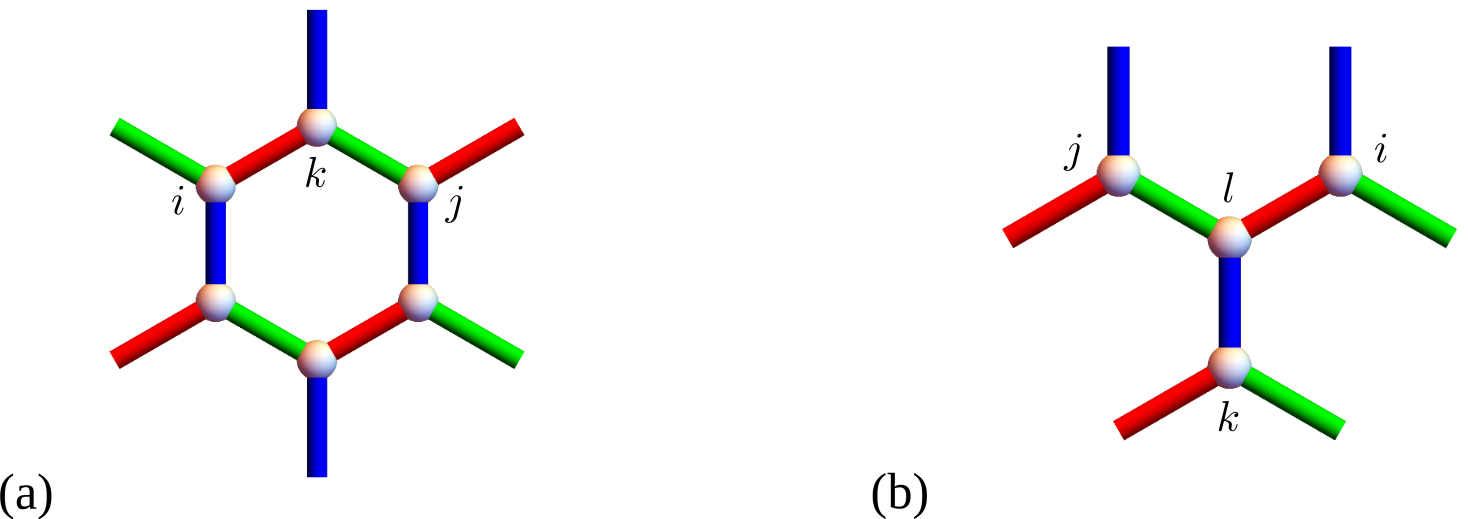
\includegraphics[width=0.8\linewidth]{./chapter02/ThreeSpinTerms.pdf}
	\caption{
		Graphical representation of third-order perturbation theory terms for the Kitaev Hamiltonian with an applied magnetic field.
		(a) Representation of the three-spin term $\sigma_i^x \sigma_j^y \sigma_k^z$ resulting in a next-nearest neighbor fermion hopping term.
		(b) Representation of the three-spin term $\sigma_i^x \sigma_j^y \sigma_k^z$ resulting in a four-fermion interaction term.
	}
	\label{fig:chapter02_ThreeSpinTerms}
\end{figure}
%

The remaining terms in Figure~\ref{fig:chapter02_ThreeSpinTerms} (a) may be reduced to Majorana bilinears resulting in next-nearest-neighbor hopping terms
%
\begin{equation}
	\op{\Sigma}_{\rm (a)} = \sum_{(i,j,k)} i \kappa \epsilon^{\alpha\beta\gamma} \op{D}_k \op{u}_{ik} \op{u}_{kj} c_i c_j,
	\label{eq:chapter02_HeffGauge}
\end{equation}
%
where the sum is over unordered triples $(i,j,k)$ of the type appearing in Figure~\ref{fig:chapter02_ThreeSpinTerms} (a) and where the intra-sublattice hopping strength $\kappa \sim \frac{h_x h_y h_z}{J^2}$ is determined by virtual flux excitations.
More precisely, $\kappa \approx 6\frac{h_x h_y h_z}{(0.27 J)^2}$ for the case presented here\footnote{The factor of $6$ is a combinatorial prefactor accounting for the fact that the sum in Eq.~\eqref{eq:chapter02_HeffGauge} occurs over \textit{unordered} triples.} on the honeycomb lattice~\cite{KitaevAoP2006}, however, the energy cost of virtual flux excitations depends on the lattice under consideration and the exact way in which the fluxes are excited~\cite{OBrienPRB2016}, as is shown in Chapter~\ref{chapter:ClassificationOfKSL} where generalizations of the Kitaev honeycomb model to other lattices are treated.

While the effective Hamiltonian~\eqref{eq:chapter02_HeffGauge} can be seen to mix different gauge sectors, as one wishes to work in the physical, \ie, gauge symmetrized, space, it shall henceforth be restricted to a fixed gauge.
Again choosing a translationally invariant gauge, the full Hamiltonian may be written in momentum space as
%
\begin{equation}
	H(\bk) = -\mathfrak{Im}[f(\bk)] \tau^x - \mathfrak{Re}[f(\bk)] \tau^y + \Delta(\bk) \tau^z,
	\label{eq:chapter02_KitaevHamiltonianMagnetic}
\end{equation}
%
where the mass term is given by
%
\begin{equation}
	\Delta(\bk) = 4\kappa \big(\sin{(\bk \cdot \ba_1)} - \sin{(\bk \cdot \ba_2)} + \sin{(\bk \cdot (\ba_1 - \ba_2))}\big).
\end{equation}
%
Here it can be seen how the breaking of time-reversal symmetry in physical spin space leads to the breaking of time-reversal symmetry in the fermionic Hamiltonian, signaled concretely by the breaking of sublattice symmetry.
The resulting dispersion of the fermionic excitations in the presence of a magnetic field
%
\begin{equation}
	E(\bk) = \pm \sqrt{|f(\bk)|^2 + |\Delta(\bk)|^2}
\end{equation}
%
is now seen to posses an energy gap of $2\Delta(\bk^*)$, where $\bk^*$ corresponds to the momentum at which a Dirac node was located before the application of the magnetic field.


%
%
%%%%%%%%%%%%%%%%%%%%%%%%%%%%%%%%%%%%%%%%%%%%%%%%%%%%%%%%%%%%%%%%%%%%%%%%%%%%%%%%%%%%%%%%
\subsection{Topology of the effective Hamiltonian}
%%%%%%%%%%%%%%%%%%%%%%%%%%%%%%%%%%%%%%%%%%%%%%%%%%%%%%%%%%%%%%%%%%%%%%%%%%%%%%%%%%%%%%%%
%
%
%
\begin{figure}[tb]
	\centering
	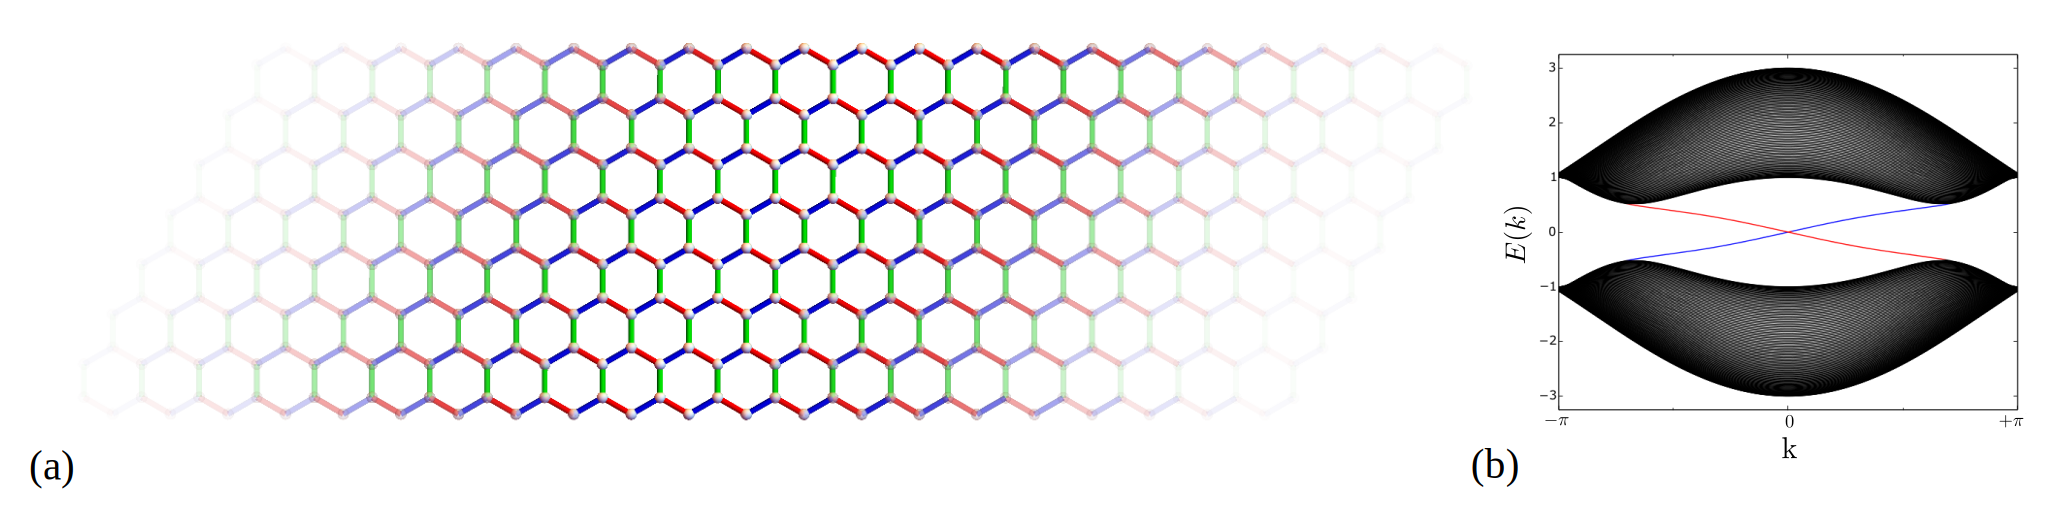
\includegraphics[width=\linewidth]{./chapter02/ChiralEdgeModes.pdf}
	\caption{
		(a) Example slab geometry with open boundary conditions in the $\ba_2$ direction.
		(b) Spectrum of the effective Hamiltonian~\eqref{eq:chapter02_HeffGauge} for a weak magnetic field on a slab geometry.
		The fully gapped bulk bands are depicted in black.
		The left- and right-moving chiral edge modes, depicted in red and blue, respectively, are localized to opposite edges of the sample and are due to the non-trivial topology of the band structure signaled by a non-vanishing first Chern number.
	}
	\label{fig:chapter02_EdgeModes}
\end{figure}
%
When framed as a free fermion Hamiltonian, the pure Kitaev model on the honeycomb lattice corresponds to a Hamiltonian matrix in the Altland-Zirnbauer symmetry class BDI~\cite{ZirnbauerJMP1996,AltlandPRB1997}.
In this context, symmetry class BDI is defined as the class of all Hamiltonian matrices possessing time-reversal symmetry, particle-hole symmetry and sublattice symmetry, such that the time-reversal and particle-hole operators both square to the positive identity operator.
Free fermion Hamiltonians belonging to symmetry class BDI are well known to be topologically trivial in two dimensions~\cite{KitaevAIP2009,RyuNJP2010,WenPRB2012}.

However, having now simultaneously broken both time-reversal and sublattice symmetries while retaining particle-hole symmetry (squaring to $+\id$), the resulting free fermion Hamiltonian resides in symmetry class D.
Gapped free fermion Hamiltonians belonging to symmetry class D in two dimensions may be identified by an integer topological invariant known as the first Chern number~\cite{KitaevAIP2009,RyuNJP2010,WenPRB2012} (often shortened to just "Chern number" in this context).
The Chern number corresponds to the quantized total amount of Berry flux through the Brillouin zone and is well known to be an important quantity in the theory of the integer quantum Hall effect~\cite{ThoulessPRL1982,AvronPRL1983,BellissardJMP1994}.
It may be calculated directly from the eigenstates of the Hamiltonian as, \eg,
%
\begin{equation}
	\nu = \frac{1}{2\pi i} \int_{BZ} \trace{(P~dP \wedge dP)},
\end{equation}
%
where $P$ is the projector onto the negative energy states and the integral is over the entire first Brillouin zone.

The negative energy band of Hamiltonian~\eqref{eq:chapter02_KitaevHamiltonianMagnetic} can be shown to have a non-vanishing Chern number $\nu = 1$, distinguishing it as a topological Chern insulator rather than a trivial band insulator.
An observable consequence of this non-trivial topology is the existence of $\nu$ chiral gapless edge modes~\cite{HalperinPRB1982,HatsugaiPRL1993,SchulzBaldesJPA2000,KellendonkRMaP2002} (see Figure~\ref{fig:chapter02_EdgeModes}).
As will be discussed in Chapter~\ref{chapter:TransitionMetalOxides}, the Kitaev Hamiltonian may be viewed as an effective Hamiltonian of a Mott insulator and contains no electric charge carrying degrees of freedom, however, the chiral edge modes can carry a \textit{thermal} Hall current
%
\begin{equation}
	I = \frac{\pi}{24} \nu T^2
\end{equation}
%
for a small temperature gradient $T$ applied perpendicular to the sample's surface~\cite{KanePRB1997,CapelliNPB2002,KitaevAoP2006}.

Another consequence of the non-trivial topology is the presence of non-Abelian anyon excitations.
The non-Abelian statistics is due to the fact that, for non-\linebreak vanishing Chern number $\nu$, \ZZ~flux excitations carry a single, unpaired Majorana mode~\cite{KitaevAoP2006,LahtinenAoP2008}.


%
%
%%%%%%%%%%%%%%%%%%%%%%%%%%%%%%%%%%%%%%%%%%%%%%%%%%%%%%%%%%%%%%%%%%%%%%%%%%%%%%%%%%%%%%%%
\section{Summary}
\label{section:chapter02_Summary}
%%%%%%%%%%%%%%%%%%%%%%%%%%%%%%%%%%%%%%%%%%%%%%%%%%%%%%%%%%%%%%%%%%%%%%%%%%%%%%%%%%%%%%%%
%
%
Section~\ref{section:chapter02_Definition} introduces Kitaev's honeycomb model of interacting quantum spins and identifies a macroscopic number of conserved quantities defined by certain products of spins around the hexagonal plaquettes of the lattice.
In Section~\ref{section:chapter02_Z2GaugeTheory}, a representation of the spins in terms of Majorana operators is used to reframe the model as a theory of Majorana fermions coupled to a static \ZZ~gauge field.
The conserved quantities in Section~\ref{section:chapter02_Definition} are seen to correspond to the gauge fluxes in the Majorana representation and allow for an exact solution of the model.
Section~\ref{section:chapter02_GeneralAspects} discusses some general aspects of the solution including how to use Lieb's theorem to fix the ground state flux sector.
The full solution to the model is carried out in Section~\ref{section:chapter02_GroundstatePhaseDiagram}, establishing a ground state phase diagram which exhibits both gapped and gapless quantum spin liquid ground states.
While the gapped spin liquid phase is not discussed in detail in this work, the latter is seen to possess gapless fermionic excitations with a graphene-like dispersion.
In Section~\ref{section:chapter02_WeakMagneticField}, the effects of time-reversal symmetry breaking are explored both in general and in particular using a weak external magnetic field.
The Dirac fermions of the gapless phase are seen to be protected by the presence of time-reversal symmetry and are gapped out by an infinitesimal magnetic field, resulting in a topological Chern insulator.

In Chapter~\ref{chapter:ClassificationOfKSL}, Kitaev's honeycomb model is extended to a number of tricoordinated lattices in three-dimensions.
The tricoordination of these lattices ensures that an exact solution is possible, just as in the case of the two-dimensional honeycomb lattice discussed above.
Analogous to the original model, the Kitaev models defined on these lattices similarly exhibit both gapped and gapless spin liquid ground states.
The gapless fermionic excitations in these systems are seen to be very diverse, depending intimately on the geometry of a given lattice.
Chapter~\ref{chapter:ProjectiveSymmetryGroup} introduces an object called the \textit{projective symmetry group} in order to better understand the hidden order of quantum phases such as the spin liquid phase seen, \eg, in the Kitaev honeycomb model.
These ideas are shown to provide an understanding of the appearance and stability of these excitations in both the two- and three-dimensional Kitaev models.